\part{Derivatives}

\chapter{The First Principles}

\section{The First Principles}

The equation of a line $ y = mx + b $ where $ b $ is the y-intercept and $ m $ is the slope of the line. Calculating the slope is easy using any two points on the line $ (x_1, y_1) $ and $ (x_2, y_2) $. \\

\begin{theorem}[Slope]
    \begin{align}
        m
        = {\Delta y \over \Delta x}
        = {{y_2 - y_1} \over {x_2 - x_1}}
            = {f(x_2) - f(x_1) \over x_2 - x_1}
            = {f(x + h) - f(x) \over h}
    \end{align}
\end{theorem}

\begin{figure}[H]
    \centering
    \begin{tikzpicture}[scale=0.9]
        \draw[->] (-4,0) -- (4,0) node[right] {$ x $};
        \draw[->] (0,-1) -- (0,6) node[above] {$ y $};
        \draw[very thick,color=red,domain=-2:2] plot (\x,{(\x) ^ 2 + 1});
        \draw[very thick,color=blue] (-0.2,0.4)--(2,4.7);
        \node at (0.15,1.04) [red,circle,fill,inner sep=1.5pt]{};
        \node at (1.85,4.4) [red,circle,fill,inner sep=1.5pt]{};
        \draw[-,very thick] (0.15,0) -- (0.15,-0.1) -- (1.85,-0.1) -- (1.85, 0) node[below] {$ h $};
    \end{tikzpicture}
    \caption{secant line}
\end{figure}

What if we made the point even closer to $ (x, f(x)) $? \\

\begin{figure}[H]
    \centering
    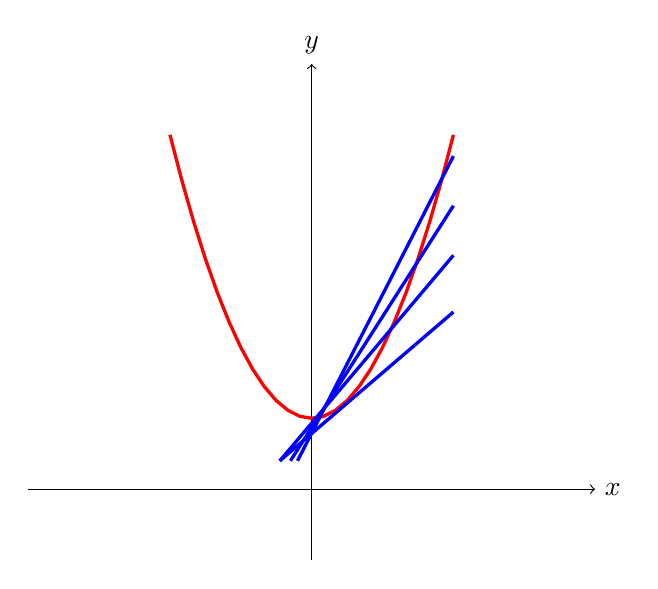
\begin{tikzpicture}[scale=0.9]
        \draw[->] (-4,0) -- (4,0) node[right] {$ x $};
        \draw[->] (0,-1) -- (0,6) node[above] {$ y $};
        \draw[very thick,color=red,domain=-2:2] plot (\x,{(\x) ^ 2 + 1});
        \draw[very thick,color=blue] (-0.2,0.4)--(2,4.7);
        \draw[very thick,color=blue] (-0.3,0.4)--(2,4);
        \draw[very thick,color=blue] (-0.45,0.4)--(2,3.3);
        \draw[very thick,color=blue] (-0.45,0.4)--(2,2.5);
    \end{tikzpicture}
    \caption{tangent line}
\end{figure}

As $ h $ gets smaller and smaller, the point $ (x+h, f(x+h)) $ approaches the point $ (x, f(x)) $. As this occurs, the slope of the secant line approaches the slope of the tangent line. We can write this action mathematically as: \\

\begin{theorem}[The First Principles]
    \begin{align}
        \lim\limits_{h \rightarrow 0}{f(x+h) - f(x) \over h}
    \end{align}
\end{theorem}

If this limit exists as a finite number, the this value is equal to the slope of the tangent line. This is the instantaneous rate of $ f(x) $ at the point $ (x, f(x)) $. This very special limit is also called the derivative of $ f(x) $ at $ (x, f(x)) $. \\

If $ y = f(x) $, then we can denote the derivative in a few different ways:

\begin{align}\nonumber
    {dy \over dx} &  & y' &  & f'(x)
\end{align}

When $ f(x) $ has a derivative at $ (a, f(a)) $, we say that $ f(x) $ is differentiable at the value $ x = a $. This means that \\

\begin{theorem}[The First Principles]
    \begin{align}
        \lim\limits_{h \rightarrow 0^-}{f(x+h) - f(x) \over h} = \lim\limits_{h \rightarrow 0^+}{f(x+h) - f(x) \over h}
    \end{align}
\end{theorem}

\begin{exercise}\nonumber
    From The First Principles, find the derivatives. \\

    (a) $ f(x) = x^2 $
    \vspace{7cm}
    \\

    (b) $ f(x) = \sqrt{x+2} $
    \vspace{9cm}
\end{exercise}

\begin{exercise}\nonumber
    From The First Principles, find the derivative of $ f(x) = {1 \over x} $ at $ x = 5 $. \\

    \begin{align}
        \\
        \\
        \\
        \\
        \\
        \\
        \\
        \\
        \\
        \\
        \\
        \\
    \end{align}
\end{exercise}

\chapter{Differentiability and Continuity}

\section{Differentiability and Continuity}

A non-differentiable function has one of the following properties: \\

\begin{figure}[H]
    \centering
    \begin{tikzpicture}[scale=0.6]
        \draw[->] (-4,0) -- (4,0) node[right] {$ x $};
        \draw[->] (0,-2) -- (0,4) node[above] {$ y $};
        \draw[very thick,color=red,domain=-3:0] plot (\x,{-\x});
        \draw[very thick,color=red,domain=0:3] plot (\x,{\x});
    \end{tikzpicture}
    \caption{corner}
\end{figure}

\begin{figure}[H]
    \centering
    \begin{tikzpicture}[scale=0.6]
        \draw[->] (-2,0) -- (4,0) node[right] {$ x $};
        \draw[->] (0,-2) -- (0,4) node[above] {$ y $};
        \draw[-,very thick,red] (0,0) -- (1.5,1) -- (2,4);
    \end{tikzpicture}
    \caption{sudden turn}
\end{figure}

\begin{figure}[H]
    \centering
    \begin{tikzpicture}[scale=0.6]
        \draw[->] (-2,0) -- (4,0) node[right] {$ x $};
        \draw[->] (0,-2) -- (0,4) node[above] {$ y $};
        \draw[-,very thick,red] (0,0) -- (1.5,1) -- (2,4);
    \end{tikzpicture}
    \caption{asymptote}
\end{figure}

\begin{figure}[H]
    \centering
    \begin{tikzpicture}[scale=0.6]
        \draw[->] (-5,0) -- (4,0) node[right] {$ x $};
        \draw[->] (0,-4) -- (0,4) node[above] {$ y $};
        \draw[very thick,color=red,domain=-4.5:-1.3] plot (\x,{1 / (\x + 1)});
        \draw[very thick,color=red,domain=-0.7:3] plot (\x,{1 / (\x + 1)});
        \draw[very thick,densely dashed,color=red] (-1,4)--(-1,-4);
    \end{tikzpicture}
    \caption{asymptote}
\end{figure}

\begin{figure}[H]
    \centering
    \begin{tikzpicture}[scale=0.6]
        \draw[->] (-5,0) -- (4,0) node[right] {$ x $};
        \draw[->] (0,-4) -- (0,4) node[above] {$ y $};
        \draw[very thick,color=red,domain=-3.5:-1.1] plot (\x,{-0.7 * (\x + 1) + 2});
        \draw[very thick,color=red,domain=-0.9:2.3] plot (\x,{(\x) ^ 2 - 2});
        \node at (-1,2) [red,circle,inner sep=1.5pt]{$\circ$};
        \node at (-0.9,-1.1) [red,circle,fill,inner sep=1.5pt]{};
    \end{tikzpicture}
    \caption{left-hand limit $ \neq $ right-hand limit}
\end{figure}

In all of these cases, the limit of the slopes does not exist at a point. Functions are not differentiable at such points. \\

Differentiability implies continuity, but the reverse is not true. Consider the function $ y = |x| $ as a counterexample. This function is continuous for all values of $ x $, but it is not differentiable at $ x = 0 $, because there is a corner there. The limit of the slopes does not exist at $ x = 0$. \\

\begin{exercise}\nonumber
    Discuss the continuity and differentiability. \\

    \begin{figure}[H]
        \centering
        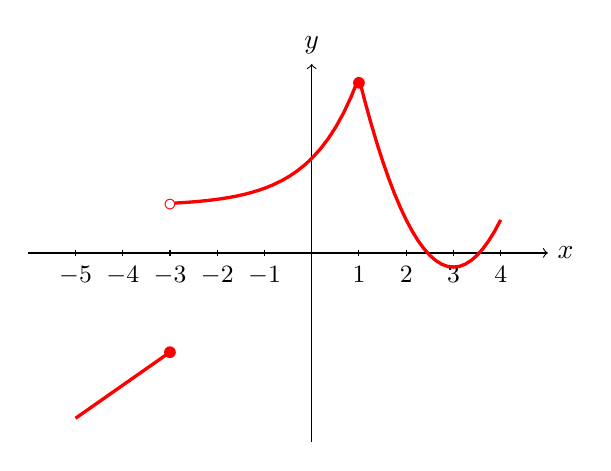
\begin{tikzpicture}[scale=0.6]
            \draw[->] (-6,0) -- (5,0) node[right] {$ x $};
            \draw[->] (0,-4) -- (0,4) node[above] {$ y $};
            \foreach \x/\xtext in {-5/-5,-4/-4,-3/-3,-2/-2,-1/-1,1/1,2/2,3/3,4/4}
            \draw[shift={(\x,0)}] (0pt,2pt) -- (0pt, -2pt) node[below] {\small $\xtext$};
            \draw[very thick,color=red,domain=-5:-3] plot (\x,{0.7 * \x});
            \draw[very thick,color=red,domain=-2.9:1] plot (\x,{e ^ \x + 1});
            \draw[very thick,color=red,domain=1:4] plot (\x,{(\x - 3) ^ 2 - 0.3});
            \node at (-3,-2.1) [red,circle,fill,inner sep=1.5pt]{};
            \node at (-3,1) [red,circle,inner sep=1.5pt]{$\circ$};
            \node at (1,3.6) [red,circle,fill,inner sep=1.5pt]{};
        \end{tikzpicture}
    \end{figure}

    (a) $ x = 2 $: \\

    (b) $ x = 1 $: \\

    (c) $ x = -3 $:
\end{exercise}

\chapter{Derivative Rules}

\section{Derivative Rules}

The First Principles definition of the limit can become a cumbersome task when functions get complicated. Luckily, there are rules for finding derivatives more quickly depending on their form. All of these rules are derived from The First Principles. \\

\subsection{Power Rule}

\begin{theorem}[Power Rule]
    Let $ f(x) = x^n $, then $ f'(x) = nx^{n-1} $.
\end{theorem}

\begin{exercise}\nonumber
    Find the derivative of $ f(x) = x^7 $.

    \vspace{1cm}
\end{exercise}

\subsection{Derivative of a Constant}

\begin{theorem}[Derivative of a Constant]
    Let $ f(x) = k $, then $ f'(x) = 0 $. Graphically, since a constant function is a horizontal line, so its slope must be zero.
\end{theorem}

\begin{exercise}\nonumber
    Find the derivative of $ f(x) = 672 $.

    \vspace{1cm}
\end{exercise}

\subsection{Derivatives of Logarithmic Functions}

\begin{theorem}[Derivatives of Logarithmic Functions]
    \begin{align}
         & {d \over dx}log_a{x} = {1 \over xln(a)},\ where\ a > 0\ and\ a \neq 1     \\
         & {d \over dx}ln(x) = {d \over dx}log_e(x) = {1 \over xln(e)} = {1 \over x}
    \end{align}
\end{theorem}

\begin{exercise}\nonumber
    Find the derivative of $ f(x) = log_4(x) $.

    \vspace{1cm}
\end{exercise}

\subsection{Derivatives of Exponential Functions}

\begin{theorem}[Derivatives of Exponential Functions]
    \begin{align}
         & {d \over dx}a^x = a^xln(a),\ where\ a > 0\ and\ a \neq 1 \\
         & {d \over dx}e^x = e^xln(e) = e^x
    \end{align}
\end{theorem}

\begin{exercise}\nonumber
    Find the derivative of $ f(x) = 5^x $.

    \vspace{1cm}
\end{exercise}

\subsection{Derivatives of Trigonometric Functions}

\begin{theorem}[Derivatives of Trigonometric Functions]
    \begin{align}
        {d \over dx}sin(x) & = cos(x)        \\
        {d \over dx}csc(x) & = -csc(x)cot(x) \\
        {d \over dx}cos(x) & = -sin(x)       \\
        {d \over dx}sec(x) & = sec(x)tan(x)  \\
        {d \over dx}tan(x) & = sec^2(x)      \\
        {d \over dx}cot(x) & = -csc^2(x)
    \end{align}
\end{theorem}

Memory tool: if the trigonometric function starts with "c" then its derivative has a minus sign. \\

What about combining these basic derivative rules for functions? That is, how do we find the derivatives of the addition, subtraction, multiplication, division, or take the constant of functions? For all of the following rules, we assume that f and g are differentiable on their domains. \\

\subsection{Multiplication by a Constant}

\begin{theorem}[Multiplication by a Constant]
    \begin{align}
        (kf(x))' = kf'(x)
    \end{align}
\end{theorem}

\begin{exercise}\nonumber
    Find the derivative of $ f(x) = 5ln(x) $.

    \vspace{1cm}
\end{exercise}

\subsection{Sum / Difference}

\begin{theorem}[Sum / Difference]
    \begin{align}
        (f \pm g)'(x) = f'(x) \pm g'(x)
    \end{align}
\end{theorem}

\begin{exercise}\nonumber
    Find the derivative of $ f(x) = ln(x) + 4x^3 - 6csc(x) $.

    \begin{align}
        \\
        \\
    \end{align}
\end{exercise}

\subsection{Product Rule}

\begin{theorem}[Product Rule]
    \begin{align}
        (fg)'(x) = f'(x)g(x) + f(x)g'(x)
    \end{align}
\end{theorem}

\begin{exercise}\nonumber
    Find the derivative of $ f(x) = ln(x)cos(x) $.

    \begin{align}
        \\
        \\
    \end{align}
\end{exercise}

\subsection{Quotient Rule}

\begin{theorem}[Quotient Rule]
    \begin{align}
        \left({f \over g}\right)'(x) = {f'g - fg' \over g^2},\ where\ g(x) \neq 0
    \end{align}
\end{theorem}

\begin{exercise}\nonumber
    Find the derivative of $ f(x) = {5^x \over x^2} $.

    \begin{align}
        \\
        \\
    \end{align}
\end{exercise}

\begin{exercise}\nonumber
    Use the Quotient Rule to prove that $ {d \over dx}cot(x) = -csc^2(x) $.

    \begin{align}
        \\
        \\
        \\
        \\
        \\
    \end{align}
\end{exercise}

\subsection{Chain Rule}

\begin{theorem}[Chain Rule]
    \begin{align}
        (f(g(x)))' = f'(g(x)) \cdot g'(x)
    \end{align}
\end{theorem}

\begin{exercise}\nonumber
    Find the derivative of the following functions. \\

    (a) $ f(x) = cos(x^3) $
    \\
    \\
    \\

    (b) $ f(x) = (x^2 + 3x + 2)^5 $
    \\
    \\
    \\

    (c) $ f(x) = ln(4x^2) $
    \\
    \\
    \\

    (d) $ f(x) = e^{sec(x)} $
    \\
    \\
    \\

    (e) $ f(x) = sin^3(x^2 + {1 \over x}) $
    \\
    \\
    \\
\end{exercise}

\chapter{Higher Order Derivatives}

\section{Higher Order Derivatives}

What happens if we take the derivative of a derivative (the second derivative)? What if we do this many times? \\

Second derivative notations:

\begin{align}\nonumber
    {d^2y \over dx^2} &  & y'' &  & f''(x)
\end{align}

Third derivative notations:

\begin{align}\nonumber
    {d^3y \over dx^3} &  & y''' &  & f'''(x)
\end{align}

Higher order derivative notations:

\begin{align}\nonumber
    {d^ny \over dx^n} &  & y^{(n)} &  & f^{(n)}(x)
\end{align}

\begin{exercise}\nonumber
    Let $ f(x) = 2x^4 $, find $ f'(x) $, $ f''(x) $, $ f'''(x) $, $ f^{(4)}(x) $, $ f^{(5)}(x) $. \\

    \begin{align}
        \\
        \\
        \\
        \\
        \\
    \end{align}
\end{exercise}

\chapter{Implicit Derivatives}

\section{Implicit Differentiation}

\begin{table}[H]
    \centering
    \begin{tabular}{| c | c | c |}
        \hline
        $ x^3 + xy + y^2 = 1 $ & $ sin(xy) + ln(x + y) = 0 $ \\ \hline
        \begin{minipage}[b]{0.5\columnwidth}
            \centering
            \raisebox{-1\height}{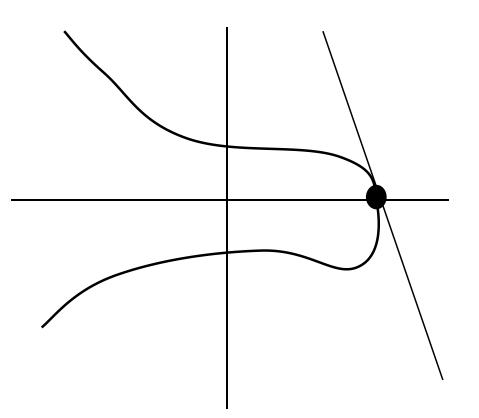
\includegraphics[width=1\linewidth]{img/part4/chapter19/1.png}}
        \end{minipage}
                               &
        \begin{minipage}[b]{0.5\columnwidth}
            \centering
            \raisebox{-1\height}{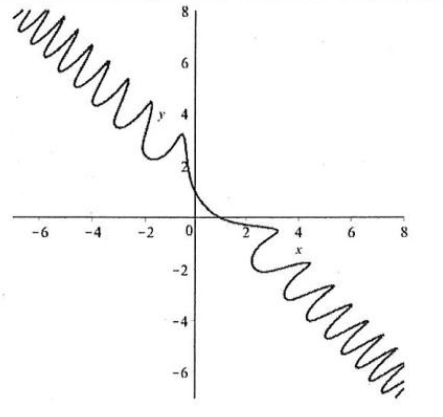
\includegraphics[width=1\linewidth]{img/part4/chapter19/2.png}}
        \end{minipage}
        \\ \hline
    \end{tabular}
\end{table}

For relations like these, there is no way to isolate for either $ x $ or $ y $. Either variable is implicitly defined in the equation in both of the above cases. \\

\begin{exercise}\nonumber
    If $ x^3 + xy + y^2 = 1 $, find $ dy \over dx $ at the point $ (x, y) = (1, 0) $. \\

    \begin{align}
        \\
        \\
        \\
        \\
        \\
        \\
        \\
        \\
    \end{align}
\end{exercise}

\begin{exercise}\nonumber
    If $ sin(tx^3) + ln(t^2 + x) = 0 $, find $ dx \over dt $. \\

    \begin{align}
        \\
        \\
        \\
        \\
        \\
        \\
    \end{align}
\end{exercise}

\begin{exercise}\nonumber
    Show that if $ e^{2xy} +e^x + e^y = y $ that $ {dx \over dy} = {1 \over {dy \over dx}} $. \\

    \begin{align}
        \\
        \\
        \\
        \\
        \\
        \\
        \\
        \\
        \\
        \\
        \\
        \\
        \\
        \\
        \\
        \\
    \end{align}
\end{exercise}

\begin{exercise}\nonumber
    If $ x^3 + x = y $, find $ d^2y \over dx^2 $. \\

    \begin{align}
        \\
        \\
        \\
        \\
        \\
        \\
        \\
        \\
        \\
        \\
        \\
    \end{align}
\end{exercise}

\begin{exercise}\nonumber
    A 10m ladder leans against a perpendicular wall. \\

    (a) The top of the ladder slides down the wall at 0.5m/s. How fast is the foot of the ladder moving at the moment the top of the ladder touches the wall 8m above the ground? \\

    \begin{figure}[H]
        \centering
        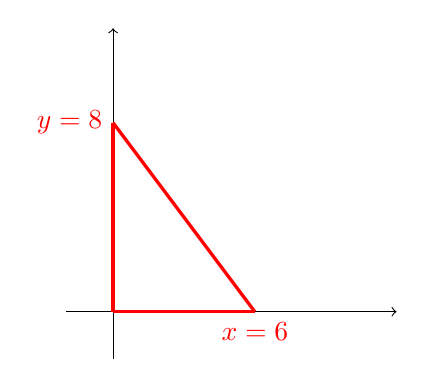
\begin{tikzpicture}[scale=0.6]
            \draw[->] (-1,0) -- (6,0);
            \draw[->] (0,-1) -- (0,6);
            \draw[-,very thick,red] (0,0) -- (3,0) node[below] {$ x = 6 $};
            \draw[-,very thick,red] (0,0) -- (0,4) node[left] {$ y = 8 $};
            \draw[-,very thick,red] (0,4) -- (3,0);
        \end{tikzpicture}
    \end{figure}

    KNOWN: $ {dy \over dt} = -0.5, y=8 $

    \begin{align}
        \\
        \\
        \\
        \\
        \\
        \\
        \\
        \\
    \end{align}

    (b) Consider the angle that the ladder makes with the ground. How fast is this angle changing at that exact moment? \\

    WANT: $ d\theta \over dt $

    \begin{align}
        \\
        \\
        \\
        \\
        \\
    \end{align}
\end{exercise}

\chapter{Logarithmic Differentiation}

\section{Logarithmic Differentiation}

Logarithmic differentiation allows us to take the derivatives of more complicated expressions. The derivative rules give us a way to quickly differentiate expression like $x^5$, $e^{4x}$, $ 2^x $. But what about $x^x$? \\

\begin{exercise}\nonumber
    Use a table of values to sketch the function $ f(x) = x^x $. \\

    \begin{figure}[H]
        \centering
        \begin{tabular}{|c|c|c|c|}
            \hline
            $ x > 0 $ & $ f(x) $ & $ x < 0 $ & $ f(x) $ \\
            \hline
                      &          &           &          \\
            \hline
                      &          &           &          \\
            \hline
                      &          &           &          \\
            \hline
                      &          &           &          \\
            \hline
        \end{tabular}
    \end{figure}

    \begin{figure}[H]
        \centering
        \begin{tikzpicture}[scale=0.6, yscale=0.7]
            \draw[->] (-2,0) -- (4,0) node[right] {$ x $};
            \draw[->] (0,-2) -- (0,7) node[above] {$ y $};
        \end{tikzpicture}
        \caption{$ y = x ^ x $ when $ x > 0 $}
    \end{figure}

    \begin{figure}[H]
        \centering
        \begin{tikzpicture}[scale=0.6]
            \draw[->] (-5,0) -- (2,0) node[right] {$ x $};
            \draw[->] (0,-3) -- (0,2) node[above] {$ y $};
        \end{tikzpicture}
        \caption{$ y = x ^ x $ when $ x < 0 $}
    \end{figure}
\end{exercise}

$ x^x $ is indeterminate when $ x = 0 $. Because the domain of $ x^x $ is extremely complicated when $ x < 0 $, this function is often only considered for $ x > 0 $. \\

So, how do we determine the derivative of this function? With logarithmic differentiation, we take the ln() of both side. Then we use log rules to simplify what we get before we finish by differentiating implicitly. \\

\begin{exercise}\nonumber
    If $ y = (cos(\pi x))^{2x} $, find $  dy \over dx $.

    \begin{align}
        \\
        \\
        \\
        \\
        \\
        \\
    \end{align}
\end{exercise}

\begin{exercise}\nonumber
    If $ y = \left(cos(\pi x)\right)^{2x} $, find $  dy \over dx $.

    \begin{align}
        \\
        \\
        \\
        \\
        \\
    \end{align}
\end{exercise}

It would be tedious to differentiate expression like $ y = {(x-2)^2(3x+1)^3\sqrt{x^2+2} \over (x-1)(x+10)^{10}} $ using product and quotient rules, and put pus at a high risk for making mistakes. We can use logarithms to simplify problems. It is technically an important step that we take the absolute value of both sides first that we aren��t considering the $ ln() $ of a negative number. \\

\begin{exercise}\nonumber
    If $ y = {(x-2)^2(3x+1)^3\sqrt{x^2+2} \over (x-1)(x+10)^{10}} $, find $ dy \over dx $. \\

    \begin{align}
        \\
        \\
        \\
        \\
        \\
        \\
        \\
        \\
        \\
        \\
        \\
        \\
    \end{align}
\end{exercise}

\chapter{Differential Approximation}

\section{Differential Approximation}

Differential approximation allows us to calculate estimates if numbers that would be impossible to find by hand. For example, we know what $ sin(\pi) $ is, but what about $ sin(3) $? \\

The idea is simple. Given a function $ f(x) $ and a difficult-to-evaluate value of $ x = a $, we want to follow this process to estimate $  f(a) $: \\

\begin{enumerate}
    \item
          Find a nearby value $ a^* $ at which $ f $ is easy to calculate. \\

    \item
          Find the tangent line there, called $ L(x) $, with slope $ f'(a^*) $. \\

    \item
          Estimate $ f(a) $ by using the height $ L(a) $ instead. \\
\end{enumerate}

\begin{figure}[H]
    \centering
    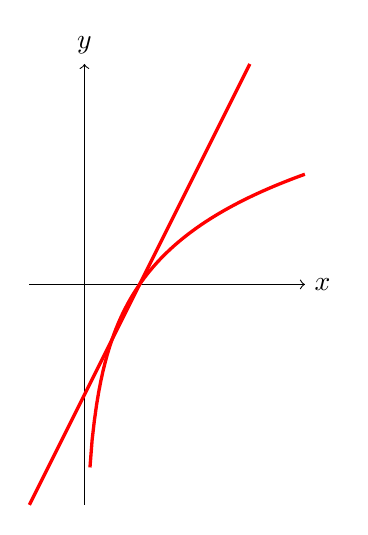
\begin{tikzpicture}[scale=0.7]
        \draw[->] (-1,0) -- (4,0) node[right] {$ x $};
        \draw[->] (0,-4) -- (0,4) node[above] {$ y $};
        \draw [very thick,color=red,domain=0.1:4,samples=100] plot (\x,{log2(\x)});
        \draw[-,red,very thick] (-1,-4) -- (3,4);
    \end{tikzpicture}
\end{figure}

\begin{exercise}\nonumber
    Estimate $ sin(3) $ using differential approximation. \\

    \vspace{8cm}
\end{exercise}

\begin{exercise}\nonumber
    Estimate $ \sqrt{65} $ using differential approximation.

    \begin{align}
        \\
        \\
        \\
        \\
        \\
        \\
        \\
        \\
        \\
        \\
        \\
        \\
        \\
        \\
        \\
        \\
    \end{align}
\end{exercise}